\documentclass[twoside]{article}%{combine}
%\usepackage{url}
\usepackage{../../tex/html}
\usepackage{epstopdf}
\usepackage{amsfonts,amsmath,color,amsthm,amssymb, enumerate, bbm, subfig}
\usepackage{graphicx}
%\usepackage[DIV=14,BCOR=2mm,headinclude=true,footinclude=false]{typearea}
%\usepackage[font=small,labelfont=bf]{caption}
\usepackage{hyperref}
\usepackage{tikz, etoolbox}

\usetikzlibrary{shapes}
\usetikzlibrary{arrows}
%\usepackage[margin=1in]{geometry}
\usepackage{graphicx,amsmath,gentium,tikz,caption}
\usetikzlibrary{patterns}
\usetikzlibrary{matrix,arrows,positioning,shapes}
\usetikzlibrary{arrows.meta}
\tikzset{
  a/.style={-{Stealth[scale=1.3,angle'=45]},semithick}
}
%\usepackage{xfrac,fontspec,unicode-math}
%\setmathfont[version=cambria]{Cambria Math}
%\mathversion{cambria}
\usepackage[letterpaper, portrait, margin=1.1in]{geometry}
\usepackage{amsmath,amsthm}
\usepackage{mathtools}
\newtheorem*{definition}{Definition}
\usepackage{tcolorbox}
\tcbset{colback=white,colframe=black}
\everymath{\displaystyle}

\makeatletter
\@ifundefined{namelength}{
\newlength{\namelength}
\settowidth{\namelength}{{\bf \Large Name: }}
\newlength{\namelinelength}
\setlength{\namelinelength}{\textwidth}
\addtolength{\namelinelength}{-\namelength}
}{}

\@ifundefined{vs}{
\newcommand*{\vs}[1]{\par
  \vspace*{#1\baselineskip}%
  \@afterindentfalse
  \@afterheading
}
}{}
\makeatother



\def\fancytitle#1#2#3{
      \centerline{\framebox{\framebox{ \parbox{.8\textwidth}{ \bf ENGRI 1101 \hfill
      Engineering Applications of OR \ \ \ \  Fall 2020 \hfill #3 #1 \\
\mbox{ }\hfill
      \hfill\mbox{ } \\[1mm] \mbox{ } \hfill{\Large \bf #2}\hfill
      \mbox{ }} }}}
      
\vs 2
}

\def\handout#1#2{\fancytitle{#1}{#2}{Handout}}
\def\review#1#2{\fancytitle{#1}{#2}{Review}}
\def\homework#1#2{\fancytitle{#1}{#2}{Homework}}
\def\exercises#1{\fancytitle{}{#1}{Exercises}}
\def\solution#1#2{\fancytitle{#1}{#2}{Solutions}}
\def\final#1#2{\fancytitle{#1}{#2}{Final}
      \noindent {\bf \Large Name:} \rule{\namelinelength}{0.5pt}
      \vspace*{\baselineskip}}
\def\prelim#1#2{\fancytitle{#1}{#2}{Prelim}
      \noindent {\bf \Large Name:} \rule{\namelinelength}{0.5pt}
      \vspace*{\baselineskip}}
\def\quiz#1#2{\fancytitle{#1}{#2}{Quiz}
      \noindent {\bf \Large Name:} \rule{\namelinelength}{0.5pt}
      \vspace*{\baselineskip}}
\def\lab#1#2{\fancytitle{#1}{#2}{Lab}
      \noindent {\bf \Large Name:} \rule{\namelinelength}{0.5pt}
      \vspace*{\baselineskip}}
\def\prelab#1#2{\fancytitle{#1}{#2}{Prelab}
      \noindent {\bf \Large Name:} \rule{\namelinelength}{0.5pt}
      \vspace*{\baselineskip}}

\raggedbottom


\begin{document}

\prelab{3}{The Minimum Spanning Tree Problem}

\noindent
\textbf{Objectives:}
\begin{itemize}
\item Introduce students to the graph theoretic concept of spanning
  trees.
\item Show three different combinatorial algorithms for solving the
  minimum spanning tree problem.
\item Demonstrate a practical use of minimum spanning trees.
\end{itemize}


\noindent 
\textbf{Optional Reading Assignment:}
\begin{itemize}
\item
Read Handout 4 on the minimum spanning tree problem.
\end{itemize}

onsider the following input for the minimum spanning tree
problem.

\begin{center}
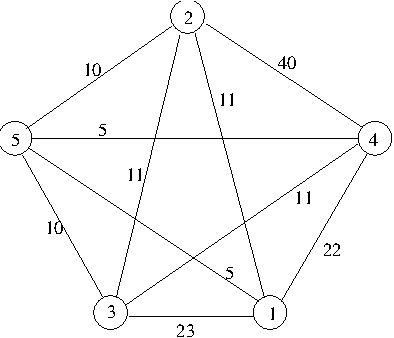
\includegraphics[height= 2in]{prelab3_fig.pdf}
\end{center}

\begin{enumerate}
\item
Find the minimum spanning tree in this graph, and give a very simple
argument why it is optimal.
\item
It turns out that our input was more complicated: only nodes 1 through
4 need to be connected. We may include node 5 if this yields a cheaper
solution, but we don't need to. Node 5 is called a {\it Steiner} node.
We wish to compute the minimum-cost tree that connects the first four
nodes. Note that this need not be a spanning tree of the graph, since
the node 5 need not be included. Find the optimal solution, and
explain why it is optimal.
\end{enumerate}



\end{document}
